In order to encode a qubit in a surface code, it suffices to define two logical
operations, namely $Z_L$ and $X_L$, which fulfill the commutation relation
$[Z_L,X_L] = 2Z_LX_L$. When multiple qubits are required, the $X_L$ and $Z_L$
operations among different qubits must commute. Figure \ref{fig:surface_code}
shows one of the possible set of physical operations that can lead to the
required logical operations. In this case, a chain of Z (X) gates in the data
qubits, represented with the red (blue) line, are one of the multiple choices to
define a logical $Z_L$ ($X_L$) operation.

However, even though a set qubits may be fully defined in terms of these
operations, it is still necessary to perform arbitrary rotations and multi-qubit
gates on them. It is a well known result of quantum computation that that it
suffices to be able to apply the standard H, T and CNOT gates to perform
universal computation. However, from Divicenzo criteria
\cite{DiCincenzoCriteria}, we see that an initialization and measurement
capabilities are also necessary.

Although all these operations can be performed using one lattice for each qubit,
is more effective to use a defect based approach. In this case, a qubit is
represented as two Z-cut (X-cut) defects, where, in its simplest form, two Z (X)
stabilizer stops participating in the QEC cycle. Figure \ref{fig:cuts} shows an
example of both Z-cut and X-cut based qubits. The figure also shows with blue
(red) line how to obtain $Z_L$ ($X_L$) operations using $Z$ ($X$) operations in
the data qubits.
\begin{figure}[htbp]
  \centering
  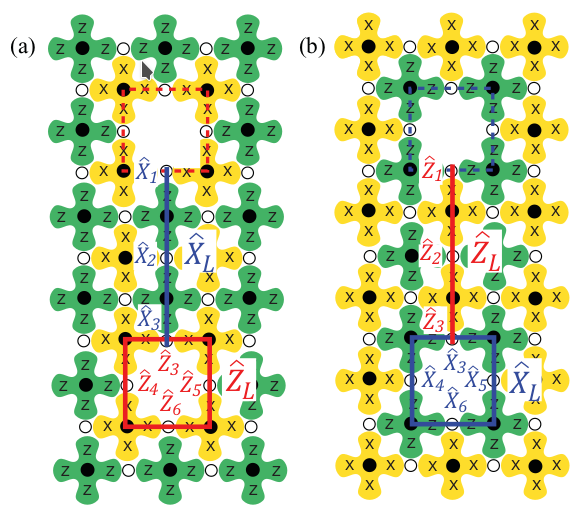
\includegraphics[width=0.5\textwidth]{images/surface_code_cuts.png}
  \caption{Examples of a Z-cut (a) and X-cut (b) qunit in a surface lattice.}
  \label{fig:cuts}
\end{figure}

These logical gates define the qubit but performing operations on them is not
straightforward. Reviewing in full detail all the operations in these defect
based qubits is far beyond the scope of this review, though there are several
techniques that we believe are worth mentioning. The first one is related to the
capability of moving the defects while preserving the state that they represent.
This can be done in several QEC cycles by means of turning off the corresponding
stabilizers and performing several measurements in the necessary data qubits. A
CNOT operation can then be performed moving one of the defects of a Z-Cut qubit
around one of the defects of an X-cut qubit. These operations are called
braiding operations and they are performed ensuring fault tolerance since the
qubits always maintain at least their initial code distance. Furthermore, every
measure explicitly performed on the data qubits can be checked with the
surrounding stabilizers to ensure fault tolerance.

The other technique that worth outlining is the implementation of and arbitrary
Z-rotation (and hence a T gate). This is performed in an indirect way by first
preparing an ancillary. Performing arbitrary rotations require the preparation
of an arbitrary state, which is by itself a challenging task. In this case, the
approach followed consist on starting with a two z-cut separated by only one
data qubit and then separating the z-cut to protect the state from the remaining
of the operation. However the final state will have a low fidelity. That is way
several states are prepared and then a purification procedure is applied, in
such a way that the high number of states are changed for the one desired state
with high fidelity.



%%% Local Variables:
%%% mode: latex
%%% TeX-master: "QEC_paper"
%%% End:
